\documentclass[12pt,a4paper]{report}
%%%%%%%%%%%%%%%%%%%%%%%%%%%%%%%%%%%%%%%%%%%%%%%%
% Language, Encoding and Fonts
% http://en.wikibooks.org/wiki/LaTeX/Internationalization
%%%%%%%%%%%%%%%%%%%%%%%%%%%%%%%%%%%%%%%%%%%%%%%%
% Select encoding of your inputs. Depends on
% your operating system and its default input
% encoding. Typically, you should use
%   Linux  : utf8 (most modern Linux distributions)
%            latin1
%   Windows: ansinew
%            latin1 (works in most cases)
%   Mac    : applemac
% Notice that you can manually change the input
% encoding of your files by selecting "save as"
% an select the desired input encoding.
\usepackage{xpatch}

%\xpretocmd{\part}{\setcounter{section}{0}}{}{}
\setcounter{secnumdepth}{4}
\usepackage[utf8]{inputenc}

% Make latex understand and use the typographic
% rules of the language used in the document.
\usepackage[english]{babel}
% Use the palatino font
%\usepackage[sc]{mathpazo}
\linespread{1.05}         % Palatino needs more leading (space between lines)
% Choose the font encoding
\usepackage[T1]{fontenc}
%%%%%%%%%%%%%%%%%%%%%%%%%%%%%%%%%%%%%%%%%%%%%%%%
% Graphics and Tables
% http://en.wikibooks.org/wiki/LaTeX/Importing_Graphics
% http://en.wikibooks.org/wiki/LaTeX/Tables
% http://en.wikibooks.org/wiki/LaTeX/Colors
%%%%%%%%%%%%%%%%%%%%%%%%%%%%%%%%%%%%%%%%%%%%%%%%
% load a colour package
\usepackage{xcolor}
\definecolor{aaublue}{RGB}{33,26,82}% dark blue
\definecolor{codegreen}{rgb}{0,0.6,0}
\definecolor{codegray}{rgb}{0.5,0.5,0.5}
\definecolor{codepurple}{rgb}{0.58,0,0.82}
\definecolor{backcolour}{rgb}{0.95,0.95,0.92}

% The standard graphics inclusion package
\usepackage{graphicx}
% Set up how figure and table captions are displayed
\usepackage{caption}
\captionsetup{%
  font=footnotesize,% set font size to footnotesize
  labelfont=bf % bold label (e.g., Figure 3.2) font
}
% Make the standard latex tables look so much better
\usepackage{array,booktabs}
% Enable the use of frames around, e.g., theorems
% The framed package is used in the example environment
\usepackage{framed}
\usepackage{csquotes}


%%%%%%%%%%%%%%%%%%%%%%%%%%%%%%%%%%%%%%%%%%%%%%%%
% Mathematics
% http://en.wikibooks.org/wiki/LaTeX/Mathematics
%%%%%%%%%%%%%%%%%%%%%%%%%%%%%%%%%%%%%%%%%%%%%%%%
% Defines new environments such as equation,
% align and split
\usepackage{amsmath}
% Adds new math symbols
\usepackage{amssymb}
% Use theorems in your document
% The ntheorem package is also used for the example environment
% When using thmmarks, amsmath must be an option as well. Otherwise \eqref doesn't work anymore.
\usepackage[framed,amsmath,thmmarks]{ntheorem}

%%%%%%%%%%%%%%%%%%%%%%%%%%%%%%%%%%%%%%%%%%%%%%%%
% Page Layout
% http://en.wikibooks.org/wiki/LaTeX/Page_Layout
%%%%%%%%%%%%%%%%%%%%%%%%%%%%%%%%%%%%%%%%%%%%%%%%
% Change margins, papersize, etc of the document
\usepackage[
  inner=28mm,% left margin on an odd page
  outer=41mm,% right margin on an odd page
  ]{geometry}
% Modify how \chapter, \section, etc. look
% The titlesec package is very configureable
\usepackage{titlesec}
%\titleformat{\chapter}[display]{\normalfont\huge\bfseries}{\chaptertitlename\ \thechapter}{20pt}{\Huge}
\titleformat*{\section}{\normalfont\Large\bfseries}
\titleformat*{\subsection}{\normalfont\large\bfseries}
\titleformat*{\subsubsection}{\normalfont\normalsize\bfseries}
%\titleformat*{\paragraph}{\normalfont\normalsize\bfseries}
%\titleformat*{\subparagraph}{\normalfont\normalsize\bfseries}

% Clear empty pages between chapters
\let\origdoublepage\cleardoublepage
\newcommand{\clearemptydoublepage}{%
  \clearpage
  {\pagestyle{empty}\origdoublepage}%
}
\let\cleardoublepage\clearemptydoublepage

% Change the headers and footers
\usepackage{fancyhdr}
\setlength{\headheight}{15pt}
\pagestyle{fancy}
% \fancyhf{} %delete everything
\renewcommand{\headrulewidth}{4pt} %remove the horizontal line in the header
\fancyhead[RE]{\small\nouppercase\leftmark} %even page - chapter title
\fancyhead[LO]{\small\nouppercase\rightmark} %uneven page - section title
\fancyhead[LE,RO]{\thepage} %page number on all pages
% Do not stretch the content of a page. Instead,
% insert white space at the bottom of the page
\raggedbottom
% % Enable arithmetics with length. Useful when
% typesetting the layout.
\usepackage{calc}

%%%%%%%%%%%%%%%%%%%%%%%%%%%%%%%%%%%%%%%%%%%%%%%%
% Bibliography
% http://en.wikibooks.org/wiki/LaTeX/Bibliography_Management
%%%%%%%%%%%%%%%%%%%%%%%%%%%%%%%%%%%%%%%%%%%%%%%%
\usepackage[backend=bibtex,
  bibencoding=utf8
  ]{biblatex}
\addbibresource{bib}
\AtBeginBibliography{\small}

%%%%%%%%%%%%%%%%%%%%%%%%%%%%%%%%%%%%%%%%%%%%%%%%
% Misc
%%%%%%%%%%%%%%%%%%%%%%%%%%%%%%%%%%%%%%%%%%%%%%%%
% Add bibliography and index to the table of
% contents
\usepackage[nottoc]{tocbibind}
% Add the command \pageref{LastPage} which refers to the
% page number of the last page
\usepackage{lastpage}
% Add todo notes in the margin of the document
\usepackage[
%  disable, %turn off todonotes
  colorinlistoftodos, %enable a coloured square in the list of todos
  textwidth=\marginparwidth, %set the width of the todonotes
  textsize=scriptsize, %size of the text in the todonotes
  ]{todonotes}

%%%%%%%%%%%%%%%%%%%%%%%%%%%%%%%%%%%%%%%%%%%%%%%%
% Gant chart
% http://en.wikibooks.org/wiki/LaTeX/gant
%%%%%%%%%%%%%%%%%%%%%%%%%%%%%%%%%%%%%%%%%%%%%%%%
\usepackage{pgfgantt}

%%%%%%%%%%%%%%%%%%%%%%%%%%%%%%%%%%%%%%%%%%%%%%%%
\usepackage{tikz}
\usetikzlibrary{calc}
%%%%%%%%%%%%%%%%%%%%%%%%%%%%%%%%%%%%%%%%%%%%%%%%
% Hyperlinks
% http://en.wikibooks.org/wiki/LaTeX/Hyperlinks
%%%%%%%%%%%%%%%%%%%%%%%%%%%%%%%%%%%%%%%%%%%%%%%%
% Enable hyperlinks and insert info into the pdf
% file. Hypperref should be loaded as one of the
% last packages
\usepackage{hyperref}
\hypersetup{%
	pdfpagelabels=true,%
	plainpages=false,%
	pdfauthor={Author(s)},%
	pdftitle={Title},%
	pdfsubject={Subject},%
	bookmarksnumbered=true,%
	colorlinks=false,%
	citecolor=black,%
	filecolor=black,%
	linkcolor=black,% you should probably change this to black before printing
	urlcolor=black,%
	pdfstartview=FitH%
}
\usepackage{enumitem}
\usepackage{adjustbox}
\usepackage{listings}
\usepackage{float}
\usepackage{multicol}
\usepackage{sectsty}
\renewcommand{\thesection}{\arabic{section}}




%\renewcommand*{\theHsection}{\theHchapter.\the\value{section}}

% Plot charts
\usepackage{pgfplots} 
\pgfplotsset{compat=1.9,
	width = 13cm,
	height = 8cm,
	ybar,
	xtick=data,
	x tick label style={font=\normalfont\tiny},
	y tick label style={font=\normalfont\tiny},
	y label style={font=\normalfont\tiny},
	legend style={font=\normalfont\tiny},
	ylabel=Time (sec),
	nodes near coords,
	nodes near coords style={
	rotate=45,
	xshift=5,
	font=\fontsize{5}{4}\selectfont,
	/pgf/number format/.cd,fixed,fixed zerofill,
	precision=3},
	ymin=0}

\definecolor{color1}{HTML}{FFB81C}
\definecolor{color2}{HTML}{C69214}
\definecolor{color3}{HTML}{F68D2E}
\definecolor{color4}{HTML}{B46A55}
\definecolor{color5}{HTML}{A4343A}
\definecolor{color6}{HTML}{565294}
\definecolor{color7}{HTML}{4F758B}
\definecolor{color8}{HTML}{285C4D}

% -- Basic formatting
\setlength{\parindent}{8pt}
\usepackage{indentfirst}


% Definig a custom style for listings:
\lstdefinestyle{mystyle}{
    backgroundcolor=\color{backcolour},   
    commentstyle=\color{codepurple},
    %keywordstyle=\color{NavyBlue},
    numberstyle=\tiny\color{codegray},
    stringstyle=\color{codepurple},
    basicstyle=\ttfamily\footnotesize\bfseries,
    breakatwhitespace=false,         
    breaklines=true,                 
    captionpos=t,                    
    keepspaces=true,                 
    numbers=left,                    
    numbersep=5pt,                  
    showspaces=false,                
    showstringspaces=false,
    showtabs=false,                  
    tabsize=2
}
% -- Setting up the custom style:
\lstset{style=mystyle}% package inclusion and set up of the document
%%%%%%%%%%%%%%%%%%%%%%%%%%%%%%%%%%%%%%%%%%%%%%%%
% Macros for the titlepage
%%%%%%%%%%%%%%%%%%%%%%%%%%%%%%%%%%%%%%%%%%%%%%%%
%Creates the aueb titlepage
\newcommand{\auebtitlepage}[3]{%
  {
    %set up various length
    \ifx\titlepageleftcolumnwidth\undefined
      \newlength{\titlepageleftcolumnwidth}
      \newlength{\titlepagerightcolumnwidth}
    \fi
    \setlength{\titlepageleftcolumnwidth}{0.5\textwidth-\tabcolsep}
    \setlength{\titlepagerightcolumnwidth}{\textwidth-12\tabcolsep-\titlepageleftcolumnwidth}
    %create title page
    \thispagestyle{empty}
    \noindent%
    \begin{tabular}{@{}ll@{}}
      \parbox{\titlepageleftcolumnwidth}{
        \includegraphics[width=0.65\paperwidth]{figures/aueb_dmst_logo}
      } &
      \parbox{\titlepagerightcolumnwidth}{\raggedleft\sf\small
        #2
      }\bigskip\\
       #1 &
      \parbox[t]{\titlepagerightcolumnwidth}{%
      \bigskip
        \fbox{\parbox{\titlepagerightcolumnwidth-2\fboxsep-2\fboxrule}{%
          #3
        }}
      }\\
    \end{tabular}
    \vfill
    \noindent{\footnotesize\emph{The content of this report is freely available, but publication (with reference) may only be pursued due to agreement with the author.}}
    \clearpage
  }
}


% my new macros
% Class options:
%-------------------------------
% nobib         - skip bibliography code/ don't include bib
% math          - include math packages and useful math commands
% hidelinks     - hide hyperref colored link boxes
% wordlinks     - link color scheme similar to word


%%%%%%%%%%%%%%%%%%%%%%%%%%%%%%%%%%%%%%%%
\begin{document}

\pdfbookmark[0]{Front page}{label:frontpage}%
\begin{titlepage}
  \title{Benchmarking big data systems for data science queries - Report}
  \author{
  Galanopoulou Rafaila 7115112200033 
  \and
  Kalopisis Giannis 7115112200011
  \and
  Notaris Giannis 7115112200038}
  \maketitle
  % \begin{center}
  %     % Words: \quickwordcount{main}\\ % Word count 
  %     % Pages: \pageref{LastPage} % Page count
  % \end{center}
% \projectinfo{}
\end{titlepage}
\clearpage

\section{Introduction}
\label{sec:intro}

This work aims to study and benchmark four widely-used 
big data systems based on their performance in handling
complex queries. More specifically, the four systems
that were selected for the benchmarking are MonetDB, 
Postgres, Vertica, and MongoDB. The evaluation is 
based on their perfomance on running queries, which
include User-Defined Functions (UDFs).

The report begins by providing background information 
for every system, as well as, an overview 
of their main features and characteristics is provided.
The benchmarking process is then presented in detail; 
including the specific UDFs that were deployed in each system, 
the performance metrics that were collected, 
and the experimental setup that was used. 
The results are presented and analyzed, 
in terms of query execution time, 
based on data overload and resource utilization. 

% The report concludes by summarizing the main findings of the study and offering recommendations for data scientists and engineers who are looking to select a big data system for their data science projects. The report also highlights the limitations of the study and suggests potential areas for future research. Overall, the report aims to provide a comprehensive and objective comparison of the performance of the four big data systems and to help data scientists and engineers make informed decisions about which system is best suited for their specific data science needs.
\section{Mongo DB}
\label{sec:mongo}

MongoDB is a popular, open-source NoSQL database management system. 
It was first released in 2009 and was created with the goal of providing a database system 
that could handle the rapidly growing amounts of data being generated by modern web applications. 
MongoDB is a \emph{document-oriented database}, not a relational one. The primary reason
for moving away from the relational model is to make scaling out easier, but there are
some other advantages as well~\cite{HPMH13}.

A document-oriented database replaces the concept of a “row” with a more flexible
model, the “document.” By allowing embedded documents and arrays, the document-oriented approach 
makes it possible to represent complex hierarchical relationships
with a single record. This fits naturally into the way developers in modern object-oriented 
languages think about their data~\cite{HPMH13}.
There are also no predefined schemas: a document’s keys and values are not of fixed
types or sizes. Without a fixed schema, adding or removing fields as needed becomes
easier. Generally, this makes development faster as developers can quickly iterate. It is
also easier to experiment. Developers can try dozens of models for the data and then
choose the best one to pursue.

MongoDB is intended to be a general-purpose database, so aside from creating, reading,
updating, and deleting data, it provides an ever-growing list of unique features:
\begin{itemize}
    \item Indexing: generic secondary indexes, allowing a variety of fast queries,
    and provides unique, compound, geospatial, and full-text indexing capabilities as
    well
    \item Aggregation: \emph{aggregation pipeline} that allows you to build complex
    aggregations from simple pieces and allow the database to optimize it.
    \item Special collection types: time-to-live collections for data that should expire at a certain
    time, such as sessions. It also fixed-size collections, which are useful for
    holding recent data, such as logs.
    \item File storage: easy-to-use protocol for storing large files and file metadata
\end{itemize}


MongoDB is powerful but easy to get started with. Some 
of the basic concepts of MongoDB:
\begin{itemize}
    \item A document is the basic unit of data for MongoDB and is roughly equivalent to a
    row in a relational database management system (but much more expressive).
    \item Similarly, a collection can be thought of as a table with a dynamic schema.
    \item A single instance of MongoDB can host multiple independent databases, each of
    which can have its own collections.
    \item Every document has a special key, "\_id", that is unique within a collection.
    \item MongoDB comes with a simple but powerful JavaScript shell, which is useful for
    the administration of MongoDB instances and data manipulation.
\end{itemize}

\section{MonetDB}
\label{sec:monet}


MonetDB is a powerful, open-source relational database management system that is optimized for analytical workloads. It uses a column-store approach, which is a different storage method than traditional row-based databases. This allows MonetDB to handle large amounts of data with high performance and efficiency. MonetDB is written in C and C++, and it supports SQL as query language. MonetDB is particularly suitable for data warehousing, business intelligence, and scientific research and it is scalable and can handle large datasets. MonetDB also supports multiple languages, including Python, making it easy to integrate with other tools and technologies.






\section{PostgreSQL}
\label{sec:postgres}


PostgreSQL is an open-source relational database management system (RD BMS) that is known for its robustness, flexibility, and scalability. It is often considered a powerful alternative to other popular RDBMSs such as MySQL and Oracle, and is used by a wide range of organizations, from small businesses to large enterprise companies. It is also a row-based database systems.

It supports the use of Python as a procedural language. This means that users can create and use Python User-Defined Functions (UDFs) within their PostgreSQL database. UDFs are custom functions that can be written in Python and used to perform a wide variety of tasks, such as data validation, data manipulation, and complex calculations. These functions can be called just like built-in PostgreSQL functions, making it easy to extend the functionality of the database. By using Python UDFs in PostgreSQL, developers can take advantage of the powerful data manipulation capabilities of Python while still utilizing the robust and reliable features of PostgreSQL.

In this work, when converting the UDFs to a suitable format for the database, not many changes were needed as PostgreSQL is smart enough to recognize that the data being entered is in array format and it executed the UDFs for each of the values of the table given to it.
\section{Vertica}
\label{sec:vertica}

In 2005, Mike Stonebraker and colleagues published a paper
outlining a formal database system, called C-store.~\cite{SABC05} 
Stonebraker formed a company "Vertica" to build a commercial 
implementation of C-Store. Vertica was acquired by HP in 2011.
% C-Store and Vertica became pioneers of a new wave of systems that 
% departed significantly from the traditional RDBMS architecture.
% Vertica became the poster child for a “NewSQL” database.
%Subsequent to the release of the C-Store model, several other significant column-based systems entered the market, including InfoBright, VectorWise, and MonetDB. 
HP Vertica was explicitly designed for analytic workloads rather than
for transactional workloads. 
HP Vertica’s free version (HP Vertica Community Edition) is Analytics Platform (currently ver. 12.0) available for download.
% in the form of a virtual machine (https://www.vertica.com/log-in/) on which operating system CentOS (64bit version) is preinstalled.
The Vertica DB physically organises table data into projections, which are sorted subsets of the attributes of a table. 
More specifically, most applications have one super projection and zero to three narrow, non-super projections. 
Each projection has a specific sort order on which the data 
is totally sorted. 
HP Vertica uses Read Optimized Store (ROS) and Write Optimized Store (WOS). 
Data in the ROS is physically stored in multiple ROS containers on a standard file system. 
Each ROS container logically contains some number of complete tuples sorted by the projection's sort order, stored as a pair of files per column. 
HP Vertica is a true column store - column files may be independently retrieved as the storage is physically separate. 
By dividing each on-disk structure into logical regions at runtime and processing the regions in parallel, HP Vertica achieves high performance.~\cite{Harr15}
\section{Evalutation}
\label{sec:experiments}

\subsection{Experimental Setup}
\subsubsection{System specifications}
\label{subsec:systemspecs}
For our experiments, we used a server with Intel i5-3470 with 3.20GHz speed. It has 4 sockets with 1 thread per socket. 
It has also 128 KiB L1d, 128 KiB L1i, 1MiB L2 and 6MiB L3 cache. Due to the CPU architecture, 
we decided in our experiments to use 1-2-4 cores/threads, 
to test parallelization, because it does not support more threads per CPU.

Regarding the memory, it has 8GB DDR3 RAM. Specifically, it has 2 dims of 4 GB each with a speed of 1333 MHz and a width of 64 bits. 
About storage, it has an SSD drive with 120 GB capacity.

\subsubsection{Query characteristics}
For benchmarking our DBS, all DBS will be evaluated in terms of performance execution of 
four queries. 
The query \textbf{311} consists of a \emph{DISTINCT} aggregate function and a 
Python UDF applied to the data. The \textbf{Weblogs} query consists mainly of a complex SELECT which 
applies most of the UDFs and a JOIN of the two datasets of the query. 
Lastly, \textbf{Zillow1} and \textbf{Zillow2} are two different queries for the same dataset. 
Zillow1 consists of nested SELECTs where the respective UDFs are applied,
and the Zillow2 query consists of many aggregate 
functions (SUM, COUNT, and GROUP BY).

\subsection{Setup DBS for experiments}
\subsubsection{PostgreSQL}
In order to run Python UDFs in PostgreSQL, we need to install the PL\/Python 
procedural language by running the command \emph{CREATE EXTENSION plpython
3u;} as a superuser in the PostgreSQL shell. 
This language allows us to write functions in Python and call them within
PostgreSQL queries. After this, we are able to run normal Python UDFs in
PostgreSQL. 
Because PostgreSQL is a row-based database, it feeds one row of data into 
each function call, so there is no need for any special changes to the 
Python code (such as the addition of iteration).

\subsubsection{MonetDB}
In order to run Python-implemented UDFs in MonetDB, we need to modify the 
configuration of the database using the command 
\emph{monetdb set embedded\_py=3 <dbname>}. 
It should be noted that this is done for each database individually within
the DBMS. Because MonetDB is a column-based database, each UDF accepts data
in the form of a table. 
Thus, we need to make a loop to pass through all the data. In traditional
row-based databases, this is not necessary, as it is done automatically by the respective DBMS.


\subsubsection{Vertica}
Python scalar UDFs in Vertica were implemented by following the steps below. 
\begin{enumerate}
	\item Install \emph{vertica\_sdk} library in the .py file.
	\item Write your Python function: The Python function should take 
	one or more inputs and return a single value, using two classes, namely
	function's class, fuction's factory class.
	\item Compile the Python function: The \emph{vertica\_sdk} library provides 
	a udf decorator that you can use to compile your Python function into a shared library.
	\item Load the shared library into Vertica: You can use the 
	\emph{CREATE OR REPLACE LIBRARY} statement to load the shared library into Vertica, 
	specifying at the end the programming language (i.e \emph{LANGUAGE Python}).
	The Library name and the path of the .py file must be specified as part of this statement.
	\item Create all python functions by using the command \emph{CREATE OR REPLACE FUNCTION}
	followed by UDF's name, programming language, name of factory class and library~\ref{lst:verticaUDF} .
\end{enumerate}
An example of a library can be found 
\href{https://www.vertica.com/docs/9.2.x/HTML/Content/Authoring/ExtendingVertica/UDx/ScalarFunctions/Python/PythonExampleAdd2Ints.htm}{here}.
\begin{lstlisting}[language=sh, caption={Example of UDF in Vertica},label={lst:verticaUDF}] 
	CREATE OR REPLACE FUNCTION extract_ip 
	AS LANGUAGE 'Python' NAME 'extract_ip_factory' 
	LIBRARY weblogslib fenced;
\end{lstlisting}

\subsubsection{MongoDB}
MongoDB is a NoSQL database and does not support executing Python functions
natively. 
However, one can execute JavaScript functions within MongoDB using the 
\emph {function} 
method, which allows one to run JavaScript code directly on the database server.
So our first alternative to run a Python function in MongoDB was to
translate it into JavaScript and then run it using \emph{function}. 
Nevertheless, that way has some limitations and is generally discouraged in production environments, 
as it can have security implications and can block the server for other operations while it's running. 
If one need to run complex logic in MongoDB, 
it's usually better to implement it outside of the database and interact with MongoDB 
using the appropriate drivers and APIs.
We used PyMongo, the Python driver for MongoDB~\footnote{\url{https://api.mongodb.com/python/current/}},
to interact with a MongoDB database from one's Python code. 
With PyMongo, one can execute operations like reading, writing, and updating documents, 
creating and managing collections, and running aggregation pipelines.


\subsection{Results}

In this section, we will present the experiments we conducted for each DBMS and analyze them. 
We chose to examine the behavior of systems with warm and cold cache memory and with the use of parallelism. 
Particularly in MongoDB, we deemed it worth comparing the performance of the Database in running UDFs using 
Pandas in Python and natively in MongoEngine (using regular expressions).

We also need to mention that measurements were made with different data volumes, 
from x1 to x128 (comparing cache until x32) from the initial size of the data, 
doubling each time the data (i.e., we have x1, x2, x4, ..., x128). 
In the following charts to better present the results and more clearly, we chose not to place all the measurements 
(however, all measurements are available for checking). Finally, each measurement is the average of 5 reputations.

\subsubsection{Cache}
\label{subsec:cache}
Reading data from disk is still much slower than reading from memories. In
order to maintain the overall speed of the system, memory is used to cache the most
recent read data, so next time when the same data is requested; the system will read
directly from memory instead of disks~\cite{Smit82}. 
To check the caching effects of the systems, every query in each DBS executed in both warm and cold cache. 
The reason for this experiment is to observe the performance of the storage systems for the environments 
with an initial state or limited memory that do not utilize the caching effect fully. 
First, cold cache is an environment where data and indexes do not reside in the memory, i.e., queries have
never been executed. 
Second, warm cache is an environment where data and indexes
reside in the memory by executing the same query prior to conducting the experiment. 
For cold cache we dropped the file systems caches using
\begin{lstlisting}[language=bash, caption= {UNIX Command for clean cache}, label={lst:paralDF}]
	echo 3 > sudo /proc/sys/vm/drop_caches
\end{lstlisting} 
before each query is performed on OS level. 
This command frees page caches in the Linux system. 

We should not expect any DBS processes to show large memory use, due to the significant small size of our datasets;
our biggest file consists of approximately 6,400,000 records, corresponds to 1.36GB. Eventually, 
warm and cold cache differences are almost insignificant. 

% You should not expect postgres processes to show large memory use, even if the whole database is cached in RAM.
% That is because PostgreSQL relies on buffered reads from the operating system buffer cache. 
% In simplified terms, when PostgreSQL does a read(), the OS looks to see whether the requested blocks are 
% cached in the "free" RAM that it uses for disk cache. If the block is in cache, the OS returns it almost instantly. 
% If the block is not in cache the OS reads it from disk, adds it to the disk cache, and returns the block.
% Subsequent reads will fetch it from the cache unless it's displaced from the cache by other blocks.

\begin{figure}[!ht]
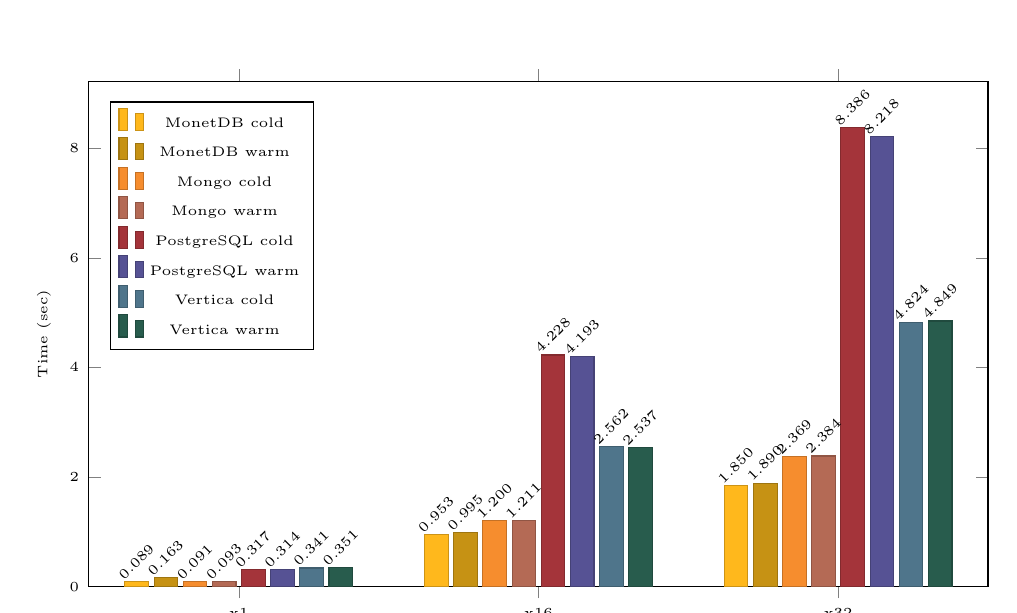
\begin{tikzpicture}
\begin{axis}[
	symbolic x coords={x1, x16, x32},
	enlarge x limits=0.25,
	legend style={at={(0.25,0.96)}, anchor=north east}
]
\addplot+ [bar width=0.3cm, ybar, color1!80!black, fill=color1, text=black] coordinates {(x1, 0.0894) (x16, 0.953) (x32, 1.8502)};
\addplot+ [bar width=0.3cm, ybar, color2!80!black, fill=color2, text=black] coordinates {(x1, 0.163) (x16, 0.995) (x32, 1.8902)};
\addplot+ [bar width=0.3cm, ybar, color3!80!black, fill=color3, text=black] coordinates {(x1, 0.0907822) (x16, 1.1996344) (x32, 2.3687442)};
\addplot+ [bar width=0.3cm, ybar, color4!80!black, fill=color4, text=black] coordinates {(x1, 0.0934848) (x16, 1.2112494) (x32, 2.3839544)};
\addplot+ [bar width=0.3cm, ybar, color5!80!black, fill=color5, text=black] coordinates {(x1, 0.3174) (x16, 4.2282) (x32, 8.3862)};
\addplot+ [bar width=0.3cm, ybar, color6!80!black, fill=color6, text=black] coordinates {(x1, 0.3136) (x16, 4.1932) (x32, 8.2184)};
\addplot+ [bar width=0.3cm, ybar, color7!80!black, fill=color7, text=black] coordinates {(x1, 0.3408) (x16, 2.5616) (x32, 4.8236)};
\addplot+ [bar width=0.3cm, ybar, color8!80!black, fill=color8, text=black] coordinates {(x1, 0.3514) (x16, 2.5368) (x32, 4.8488)};
\legend{MonetDB cold, MonetDB warm, Mongo cold, Mongo warm, PostgreSQL cold, PostgreSQL warm, Vertica cold, Vertica warm}
\end{axis}
\end{tikzpicture}
	\caption{311 (Cold/Warm cache)}
	\label{fig:311Cache}

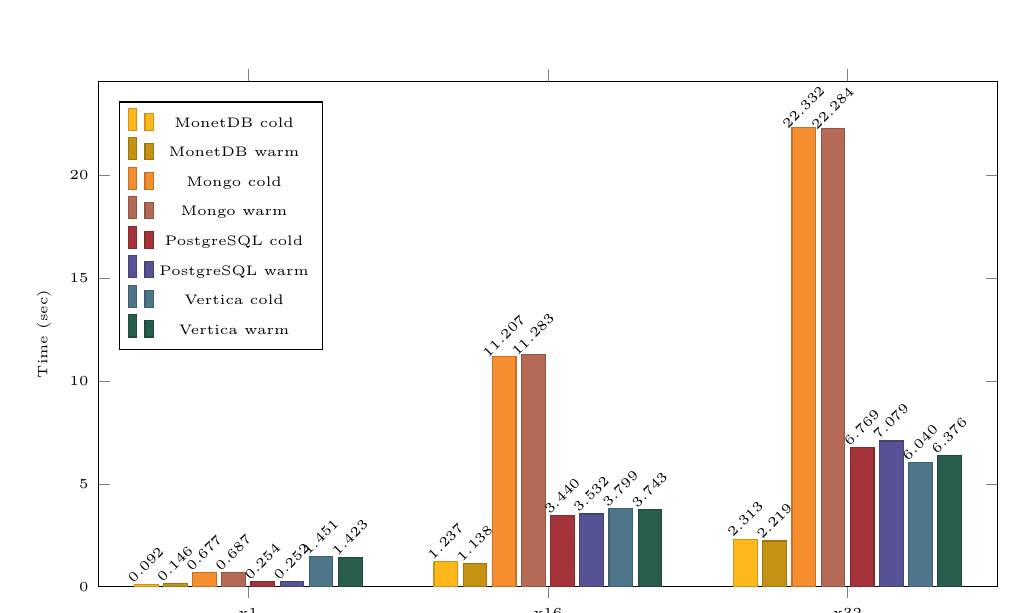
\begin{tikzpicture}
\begin{axis}[
	symbolic x coords={x1, x16, x32},
	enlarge x limits=0.25,
	legend style={at={(0.25,0.96)}, anchor=north east}
]
\addplot+ [bar width=0.3cm, ybar, color1!80!black, fill=color1, text=black] coordinates {(x1, 0.0916) (x16, 1.2374) (x32, 2.3126)};
\addplot+ [bar width=0.3cm, ybar, color2!80!black, fill=color2, text=black] coordinates {(x1, 0.1456) (x16, 1.1384) (x32, 2.2192)};
\addplot+ [bar width=0.3cm, ybar, color3!80!black, fill=color3, text=black] coordinates {(x1, 0.677313) (x16, 11.2072838) (x32, 22.3317652)};
\addplot+ [bar width=0.3cm, ybar, color4!80!black, fill=color4, text=black] coordinates {(x1, 0.6868898) (x16, 11.283492) (x32, 22.2838622)};
\addplot+ [bar width=0.3cm, ybar, color5!80!black, fill=color5, text=black] coordinates {(x1, 0.2538) (x16, 3.44) (x32, 6.7694)};
\addplot+ [bar width=0.3cm, ybar, color6!80!black, fill=color6, text=black] coordinates {(x1, 0.2516) (x16, 3.532) (x32, 7.0788)};
\addplot+ [bar width=0.3cm, ybar, color7!80!black, fill=color7, text=black] coordinates {(x1, 1.4508) (x16, 3.7988) (x32, 6.0396)};
\addplot+ [bar width=0.3cm, ybar, color8!80!black, fill=color8, text=black] coordinates {(x1, 1.4228) (x16, 3.7426) (x32, 6.3762)};
\legend{MonetDB cold, MonetDB warm, Mongo cold, Mongo warm, PostgreSQL cold, PostgreSQL warm, Vertica cold, Vertica warm}
\end{axis}
\end{tikzpicture}
	\caption{Weblogs (Cold/Warm cache)}
	\label{fig:WeblogsCache}
\end{figure}

\begin{figure}[!ht]
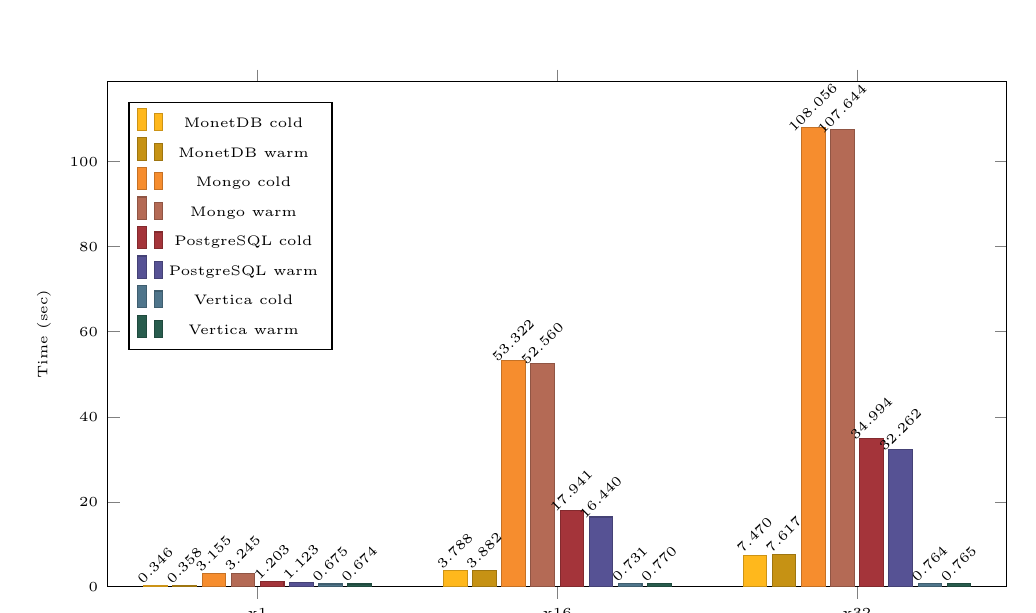
\begin{tikzpicture}
\begin{axis}[
	symbolic x coords={x1, x16, x32},
	enlarge x limits=0.25,
	legend style={at={(0.25,0.96)}, anchor=north east}
]
\addplot+ [bar width=0.3cm, ybar, color1!80!black, fill=color1, text=black] coordinates {(x1, 0.3462) (x16, 3.7882) (x32, 7.4704)};
\addplot+ [bar width=0.3cm, ybar, color2!80!black, fill=color2, text=black] coordinates {(x1, 0.3582) (x16, 3.8824) (x32, 7.6168)};
\addplot+ [bar width=0.3cm, ybar, color3!80!black, fill=color3, text=black] coordinates {(x1, 3.1553452) (x16, 53.32206) (x32, 108.055524)};
\addplot+ [bar width=0.3cm, ybar, color4!80!black, fill=color4, text=black] coordinates {(x1, 3.2449956) (x16, 52.5604554) (x32, 107.6443716)};
\addplot+ [bar width=0.3cm, ybar, color5!80!black, fill=color5, text=black] coordinates {(x1, 1.2028) (x16, 17.9406) (x32, 34.9936)};
\addplot+ [bar width=0.3cm, ybar, color6!80!black, fill=color6, text=black] coordinates {(x1, 1.1228) (x16, 16.4402) (x32, 32.262)};
\addplot+ [bar width=0.3cm, ybar, color7!80!black, fill=color7, text=black] coordinates {(x1, 0.6754) (x16, 0.7314) (x32, 0.7644)};
\addplot+ [bar width=0.3cm, ybar, color8!80!black, fill=color8, text=black] coordinates {(x1, 0.6742) (x16, 0.7704) (x32, 0.765)};
\legend{MonetDB cold, MonetDB warm, Mongo cold, Mongo warm, PostgreSQL cold, PostgreSQL warm, Vertica cold, Vertica warm}
\end{axis}
\end{tikzpicture}
	\caption{Zillow 1 (Cold/Warm cache)}
	\label{fig:Zillow1Cache}

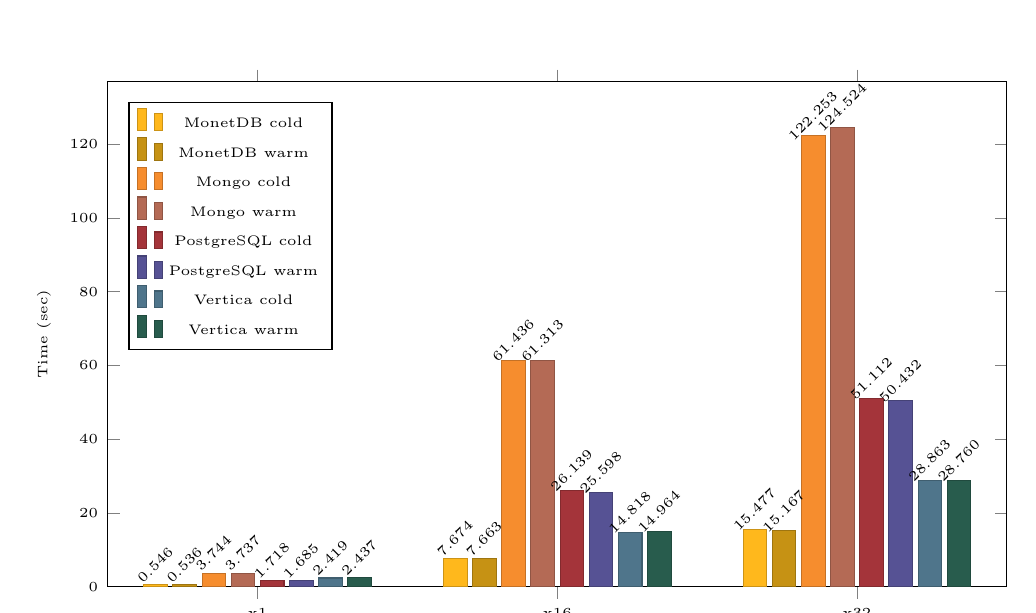
\begin{tikzpicture}
\begin{axis}[
	symbolic x coords={x1, x16, x32},
	enlarge x limits=0.25,
	legend style={at={(0.25,0.96)}, anchor=north east}
]
\addplot+ [bar width=0.3cm, ybar, color1!80!black, fill=color1, text=black] coordinates {(x1, 0.5458) (x16, 7.6736) (x32, 15.477)};
\addplot+ [bar width=0.3cm, ybar, color2!80!black, fill=color2, text=black] coordinates {(x1, 0.5362) (x16, 7.6634) (x32, 15.167)};
\addplot+ [bar width=0.3cm, ybar, color3!80!black, fill=color3, text=black] coordinates {(x1, 3.7440264) (x16, 61.4363946) (x32, 122.2530776)};
\addplot+ [bar width=0.3cm, ybar, color4!80!black, fill=color4, text=black] coordinates {(x1, 3.7367452) (x16, 61.312647) (x32, 124.5240324)};
\addplot+ [bar width=0.3cm, ybar, color5!80!black, fill=color5, text=black] coordinates {(x1, 1.7184) (x16, 26.139) (x32, 51.1124)};
\addplot+ [bar width=0.3cm, ybar, color6!80!black, fill=color6, text=black] coordinates {(x1, 1.6854) (x16, 25.5984) (x32, 50.4318)};
\addplot+ [bar width=0.3cm, ybar, color7!80!black, fill=color7, text=black] coordinates {(x1, 2.419) (x16, 14.8176) (x32, 28.8634)};
\addplot+ [bar width=0.3cm, ybar, color8!80!black, fill=color8, text=black] coordinates {(x1, 2.4372) (x16, 14.9642) (x32, 28.7596)};
\legend{MonetDB cold, MonetDB warm, Mongo cold, Mongo warm, PostgreSQL cold, PostgreSQL warm, Vertica cold, Vertica warm}
\end{axis}
\end{tikzpicture}
	\caption{Zillow 2 (Cold/Warm cache)}
	\label{fig:Zillow2Cache}
\end{figure}

\begin{figure}[!ht]
	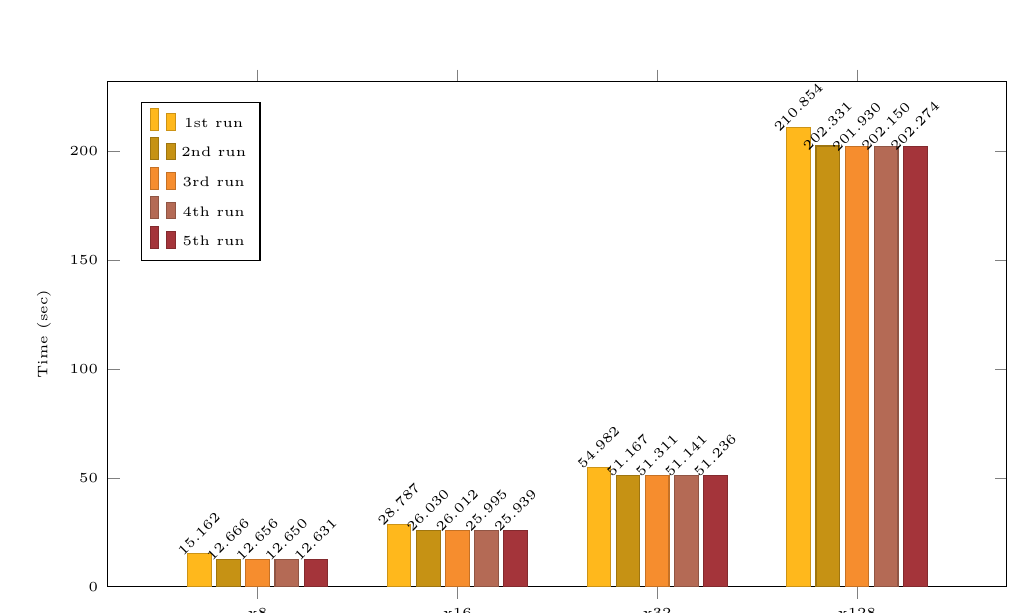
\begin{tikzpicture}
		\begin{axis}[
			symbolic x coords={x8, x16, x32, x128},
			enlarge x limits=0.25,
			legend style={at={(0.17,0.96)}, anchor=north east}
		]
		\addplot+ [bar width=0.3cm, ybar, color1!80!black, fill=color1, text=black] coordinates {(x8, 15.162) (x16, 28.787) (x32, 54.982) (x128, 210.854)};
		\addplot+ [bar width=0.3cm, ybar, color2!80!black, fill=color2, text=black] coordinates {(x8, 12.666) (x16, 26.030) (x32, 51.167) (x128, 202.331)};
		\addplot+ [bar width=0.3cm, ybar, color3!80!black, fill=color3, text=black] coordinates {(x8, 12.656) (x16, 26.012) (x32, 51.311) (x128, 201.930)};
		\addplot+ [bar width=0.3cm, ybar, color4!80!black, fill=color4, text=black] coordinates {(x8, 12.650) (x16, 25.995) (x32, 51.141) (x128, 202.150)};
		\addplot+ [bar width=0.3cm, ybar, color5!80!black, fill=color5, text=black] coordinates {(x8, 12.631) (x16, 25.939) (x32, 51.236) (x128, 202.274)};
		\legend{1st run, 2nd run, 3rd run, 4th run, 5th run}
		\end{axis}
		\end{tikzpicture}
			\caption{PostgreSQL - Zillow 2 (HDD Cache)}
			\label{fig:PostgresHDDCache}
\end{figure}


\subsubsection{Parallelization}

Starting off, we should mention again that the system we ran our experiments on consists of a 4-core processor with 1 thread per core. 
Thus, in our experiments to explore parallelism, we looked at differences between 1, 2, and 4 processes and threads. 
We chose this approach because we deemed it meaningless to use more processes/threads, as it would lead to the throttling of our machine. 
It would have been of interest to test the experiments on larger and more powerful machines and see if any differences arose 
and to what extent they are explained by the increased machine power, or to what extent the performance-to-implementation-cost ratio is satisfactory 
to make such changes.

Additionally, we consider it important to note that Python, for security reasons, allows only one thread to hold control of the Python interpreter. 
This is known as the Python Global Interpreter Lock or GIL~\cite{PythonGIL}. This is a mechanism in CPython, 
the default and most widely used implementation of the 
Python programming language, to ensure that only one thread executes Python bytecodes at a time. 
This lock is necessary because CPython's memory management is not thread-safe, meaning only one thread can be in a state of execution at any time. 
The impact of the GIL is not noticeable for developers running single-threaded programs, 
but it can be a performance bottleneck in CPU-bound and multi-threaded code. Suppose we want to write a program that needs to use multiple threads 
for maximum performance. In that case, we may consider using an alternative implementation of Python, such as Jython or IronPython, 
which do not have a GIL or use multiple processes instead of threads.

\paragraph{PostgreSQL} implements parallelism at the process level. 
This means that it could theoretically utilize the capabilities of Python 
for parallelism (as we mentioned at the beginning of the chapter) 
since Python also implements parallelism at the process level. The
parameters that we need to take into consideration in order to 
implement\/activate parallelism are:
\begin{enumerate}
	\item $max\_worker\_processes$: the maximum number of background 
	processes that the system can support.
	\item $max\_parallel\_workers\_per\_gather$: the maximum number of 
	workers that can be started by a single Gather or Gather Merge node
	\item $max\_parallel\_workers$: the maximum number of workers that the 
	system can support for parallel queries
	\item $max\_parallel\_maintenance\_workers$: the maximum number of 
	parallel workers that a single utility command can start
\end{enumerate}
Also, the $dynamic\_shared\_memory\_type$ parameter should be enabled with
the appropriate value, depending on the system that the DBMS is running on.

Below, we see the diagrams that show the results we had running the queries 
on 1, 2, and 4 cores.

\begin{figure}[!ht]
	\begin{minipage}{.5\textwidth}
	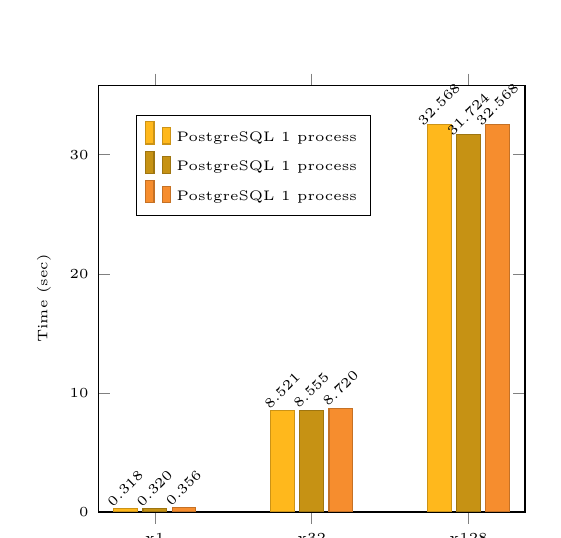
\begin{tikzpicture}
	\begin{axis}[
		symbolic x coords={x1, x32, x128},
		enlarge x limits=0.18,
		legend style={at={(0.64,0.93)}, anchor=north east},
		width = 7cm,
		height = 7cm
	]
	\addplot+ [bar width=0.3cm, ybar, color1!80!black, fill=color1, text=black] coordinates {(x1, 0.3176) (x32, 8.5206) (x128, 32.5684) };
	\addplot+ [bar width=0.3cm, ybar, color2!80!black, fill=color2, text=black] coordinates {(x1, 0.3198) (x32, 8.5554) (x128, 31.7244) };
	\addplot+ [bar width=0.3cm, ybar, color3!80!black, fill=color3, text=black] coordinates {(x1, 0.356) (x32, 8.7202) (x128, 32.5684) };
	\legend{PostgreSQL 1 process, PostgreSQL 1 process, PostgreSQL 1 process}
	\end{axis}
	\end{tikzpicture}
		\caption{PostgreSQL - 311 (Parallelism)}
		\label{fig:311ParallelismPostgreSQL}
	\end{minipage}%
	\begin{minipage}{.5\textwidth}
	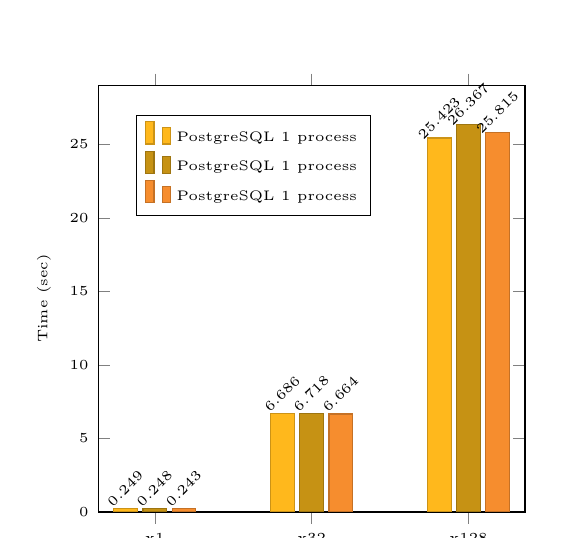
\begin{tikzpicture}
	\begin{axis}[
		symbolic x coords={x1, x32, x128},
		enlarge x limits=0.18,
		legend style={at={(0.64,0.93)}, anchor=north east},
		width = 7cm,
		height = 7cm
	]
	\addplot+ [bar width=0.3cm, ybar, color1!80!black, fill=color1, text=black] coordinates {(x1, 0.2494) (x32, 6.6864) (x128, 25.4232) };
	\addplot+ [bar width=0.3cm, ybar, color2!80!black, fill=color2, text=black] coordinates {(x1, 0.2476) (x32, 6.7178) (x128, 26.367) };
	\addplot+ [bar width=0.3cm, ybar, color3!80!black, fill=color3, text=black] coordinates {(x1, 0.2432) (x32, 6.6638) (x128, 25.8148) };
	\legend{PostgreSQL 1 process, PostgreSQL 1 process, PostgreSQL 1 process}
	\end{axis}
	\end{tikzpicture}
		\caption{PostgreSQL - Weblogs (Parallelism)}
		\label{fig:WeblogsParallelismPostgreSQL}
	\end{minipage}
	\end{figure}
	\begin{figure}[!ht]
	\begin{minipage}{.5\textwidth}
	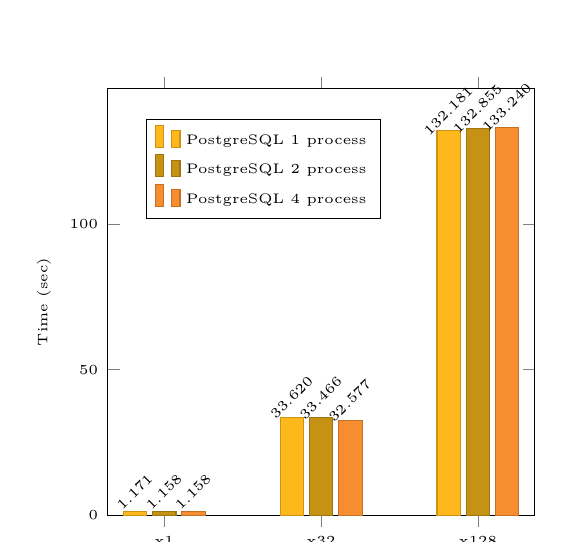
\begin{tikzpicture}
	\begin{axis}[
		symbolic x coords={x1, x32, x128},
		enlarge x limits=0.18,
		legend style={at={(0.64,0.93)}, anchor=north east},
		width = 7cm,
		height = 7cm
	]
	\addplot+ [bar width=0.3cm, ybar, color1!80!black, fill=color1, text=black] coordinates {(x1, 1.1708) (x32, 33.6204) (x128, 132.1814) };
	\addplot+ [bar width=0.3cm, ybar, color2!80!black, fill=color2, text=black] coordinates {(x1, 1.1578) (x32, 33.4664) (x128, 132.8554) };
	\addplot+ [bar width=0.3cm, ybar, color3!80!black, fill=color3, text=black] coordinates {(x1, 1.1584) (x32, 32.577) (x128, 133.2398) };
	\legend{PostgreSQL 1 process, PostgreSQL 2 process, PostgreSQL 4 process}
	\end{axis}
	\end{tikzpicture}
		\caption{PostgreSQL - Zillow1 (Parallelism)}
		\label{fig:Zillow1ParallelismPostgreSQL}
	\end{minipage}%
	\begin{minipage}{.5\textwidth}
	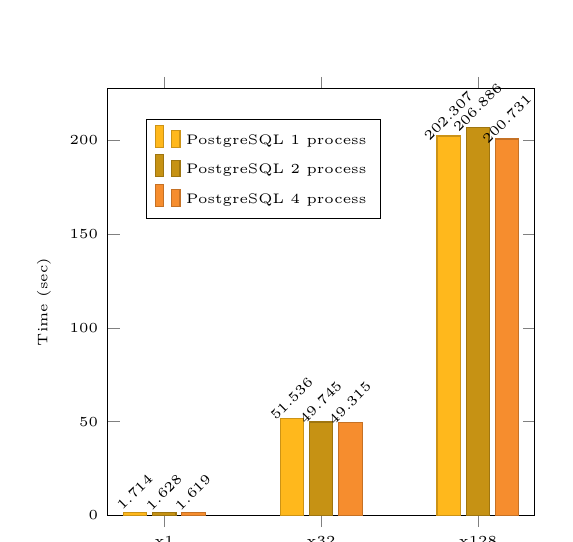
\begin{tikzpicture}
	\begin{axis}[
		symbolic x coords={x1, x32, x128},
		enlarge x limits=0.18,
		legend style={at={(0.64,0.93)}, anchor=north east},
		width = 7cm,
		height = 7cm
	]
	\addplot+ [bar width=0.3cm, ybar, color1!80!black, fill=color1, text=black] coordinates {(x1, 1.7136) (x32, 51.5364) (x128, 202.3072) };
	\addplot+ [bar width=0.3cm, ybar, color2!80!black, fill=color2, text=black] coordinates {(x1, 1.6276) (x32, 49.7454) (x128, 206.8864) };
	\addplot+ [bar width=0.3cm, ybar, color3!80!black, fill=color3, text=black] coordinates {(x1, 1.6186) (x32, 49.3152) (x128, 200.7306) };
	\legend{PostgreSQL 1 process, PostgreSQL 2 process, PostgreSQL 4 process}
	\end{axis}
	\end{tikzpicture}
		\caption{PostgreSQL - Zillow2 (Parallelism)}
		\label{fig:Zillow2ParallelismPostgreSQL}
	\end{minipage}
	\end{figure}	

\paragraph{MonetDB}
\label{par:MonetFBPar}
on the other hand, implements parallelism at thread 
level. 
That is, for the same process, it generates many threads that operate on 
the same memory, having common global variables, heap, and code. 
This is in contrast to what Python provides us, where UDFs are implemented. 
As we will see in the charts, MonetDB cannot leverage parallelism enough to
give us satisfactory results. 
Also, in the charts it shows that we tried parallelism at both thread level 
and database-pipeline level.

Regarding the thread-level parallelization, we modified the number of 
nthreads through the database configuration, using the 
\emph{monetdb set nthreads=x <dbname>} command. 
As for the pipeline method mentioned earlier, MonetDB internally implements
a type of pipeline to give a speedup in processing the data. 
The user has the option to disable it with the 
\emph{monetdb set optpipe=sequential\_pipe <dbname>} command. 
We thought it would be interesting to see how such an option affects the 
speed of our results. 
In the following charts, in the sequential pipeline, we used 4 threads 
which is the default option of MonetDB.

\begin{figure}[t]
	\begin{minipage}{.5\textwidth}
	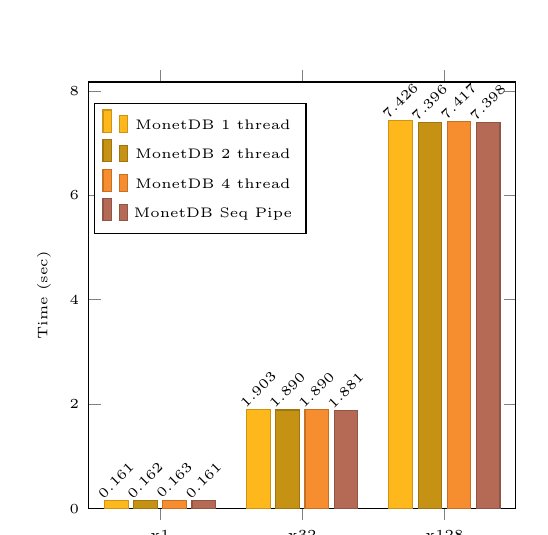
\begin{tikzpicture}
	\begin{axis}[
		symbolic x coords={x1, x32, x128},
		enlarge x limits=0.25,
		legend style={at={(0.51,0.95)}, anchor=north east},
		width = 7cm,
		height = 7cm
	]
	\addplot+ [bar width=0.3cm, ybar, color1!80!black, fill=color1, text=black] coordinates {(x1, 0.161) (x32, 1.9026) (x128, 7.4264) };
	\addplot+ [bar width=0.3cm, ybar, color2!80!black, fill=color2, text=black] coordinates {(x1, 0.1622) (x32, 1.8896) (x128, 7.3956) };
	\addplot+ [bar width=0.3cm, ybar, color3!80!black, fill=color3, text=black] coordinates {(x1, 0.163) (x32, 1.8902) (x128, 7.417) };
	\addplot+ [bar width=0.3cm, ybar, color4!80!black, fill=color4, text=black] coordinates {(x1, 0.1608) (x32, 1.8808) (x128, 7.3984) };
	\legend{MonetDB 1 thread, MonetDB 2 thread, MonetDB 4 thread, MonetDB Seq Pipe}
	\end{axis}
	\end{tikzpicture}
		\caption{MonetDB - 311 (Parallelism)}
		\label{fig:311ParallelismMonet}
	\end{minipage}%
	\begin{minipage}{.5\textwidth}
	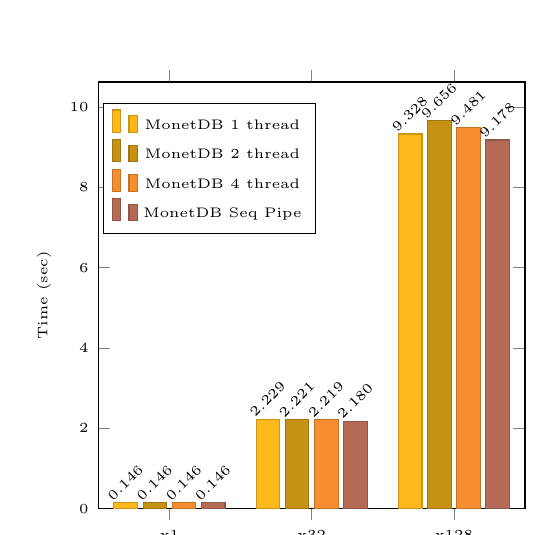
\begin{tikzpicture}
	\begin{axis}[
		symbolic x coords={x1, x32, x128},
		enlarge x limits=0.25,
		legend style={at={(0.51,0.95)}, anchor=north east},
		width = 7cm,
		height = 7cm
	]
	\addplot+ [bar width=0.3cm, ybar, color1!80!black, fill=color1, text=black] coordinates {(x1, 0.146) (x32, 2.2292) (x128, 9.328) };
	\addplot+ [bar width=0.3cm, ybar, color2!80!black, fill=color2, text=black] coordinates {(x1, 0.1464) (x32, 2.2208) (x128, 9.6558) };
	\addplot+ [bar width=0.3cm, ybar, color3!80!black, fill=color3, text=black] coordinates {(x1, 0.1456) (x32, 2.2192) (x128, 9.4814) };
	\addplot+ [bar width=0.3cm, ybar, color4!80!black, fill=color4, text=black] coordinates {(x1, 0.1464) (x32, 2.1796) (x128, 9.1778) };
	\legend{MonetDB 1 thread, MonetDB 2 thread, MonetDB 4 thread, MonetDB Seq Pipe}
	\end{axis}
	\end{tikzpicture}
		\caption{MonetDB - Weblogs (Parallelism)}
		\label{fig:WeblogsParallelismMonet}
	\end{minipage}
	\end{figure}
	\begin{figure}[t]
	\begin{minipage}{.5\textwidth}
	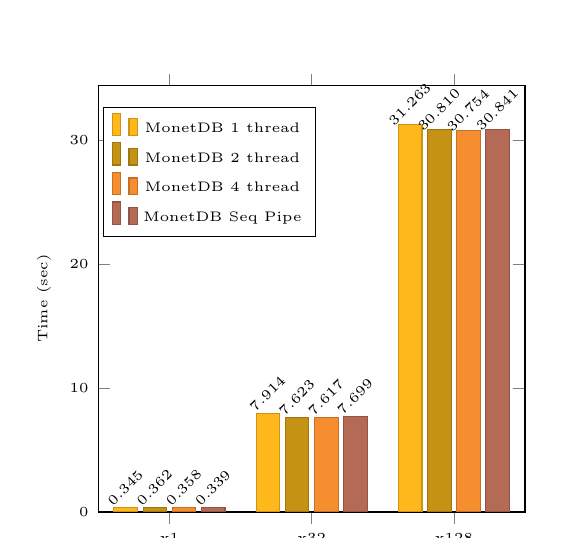
\begin{tikzpicture}
	\begin{axis}[
		symbolic x coords={x1, x32, x128},
		enlarge x limits=0.25,
		legend style={at={(0.51,0.95)}, anchor=north east},
		width = 7cm,
		height = 7cm
	]
	\addplot+ [bar width=0.3cm, ybar, color1!80!black, fill=color1, text=black] coordinates {(x1, 0.3454) (x32, 7.9144) (x128, 31.263) };
	\addplot+ [bar width=0.3cm, ybar, color2!80!black, fill=color2, text=black] coordinates {(x1, 0.3622) (x32, 7.6228) (x128, 30.8102) };
	\addplot+ [bar width=0.3cm, ybar, color3!80!black, fill=color3, text=black] coordinates {(x1, 0.3582) (x32, 7.6168) (x128, 30.754) };
	\addplot+ [bar width=0.3cm, ybar, color4!80!black, fill=color4, text=black] coordinates {(x1, 0.339) (x32, 7.6994) (x128, 30.8414) };
	\legend{MonetDB 1 thread, MonetDB 2 thread, MonetDB 4 thread, MonetDB Seq Pipe}
	\end{axis}
	\end{tikzpicture}
		\caption{MonetDB - Zillow1 (Parallelism)}
		\label{fig:Zillow1ParallelismMonet}
	\end{minipage}%
	\begin{minipage}{.5\textwidth}
	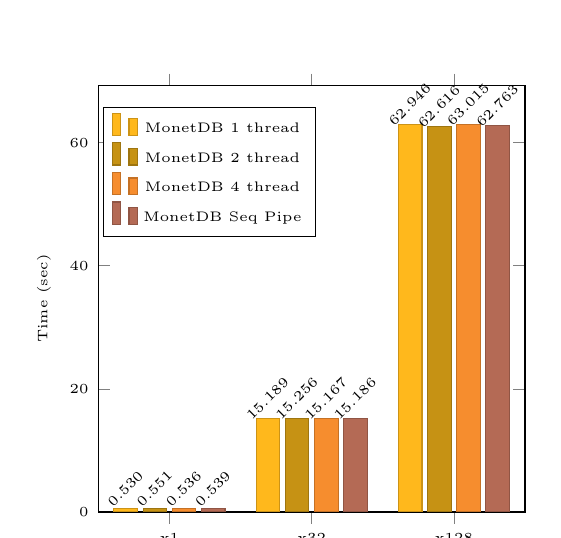
\begin{tikzpicture}
	\begin{axis}[
		symbolic x coords={x1, x32, x128},
		enlarge x limits=0.25,
		legend style={at={(0.51,0.95)}, anchor=north east},
		width = 7cm,
		height = 7cm
	]
	\addplot+ [bar width=0.3cm, ybar, color1!80!black, fill=color1, text=black] coordinates {(x1, 0.5304) (x32, 15.1888) (x128, 62.946) };
	\addplot+ [bar width=0.3cm, ybar, color2!80!black, fill=color2, text=black] coordinates {(x1, 0.5506) (x32, 15.2562) (x128, 62.6158) };
	\addplot+ [bar width=0.3cm, ybar, color3!80!black, fill=color3, text=black] coordinates {(x1, 0.5362) (x32, 15.167) (x128, 63.015) };
	\addplot+ [bar width=0.3cm, ybar, color4!80!black, fill=color4, text=black] coordinates {(x1, 0.539) (x32, 15.1864) (x128, 62.7628) };
	\legend{MonetDB 1 thread, MonetDB 2 thread, MonetDB 4 thread, MonetDB Seq Pipe}
	\end{axis}
	\end{tikzpicture}
		\caption{MonetDB - Zillow2 (Parallelism)}
		\label{fig:Zillow2ParallelismMonet}
	\end{minipage}
	\end{figure}

\paragraph{Vertica}
unlike PostgreSQL and Monet, which do not employ parallelism in the queries tested, Vertica adopts a different 
approach utilizing parallelism at both the node and cluster levels~\cite{LFVT12}.

The Vertica Execution Engine (EE) is responsible for executing all processes for the query plan. 
A query plan is represented as a tree of operations, where each operator performs a specific algorithm. 
The EE uses a multi-threaded and pipelined architecture, allowing for multiple operators to run 
concurrently and multiple threads to execute code for a single operator. Additionally, the EE is 
vectorized and requests blocks of rows instead of individual rows, similar to the C-Store database.

At the single node level, Vertica employs parallelism on a smaller scale by dividing the data locally 
and processing it in parallel to keep all cores fully utilized. For instance, multiple GroupBy operators 
run in parallel and request data from the StorageUnion~\footnote{StorageUnion is a feature in the Vertica 
database management system that provides support for data storage and retrieval across different storage media.}.

At the cluster level, Vertica divides the data across multiple nodes and executes the query in parallel 
on each node. The nodes exchange intermediate results and aggregate the final results to produce the 
final answer, resulting in a "massively parallel processing" (MPP) architecture. This architecture enables 
Vertica to efficiently handle large data volumes and complex queries in a scalable manner. In the experiments 
conducted, we created three resource pools as depicted in table~\ref{tab:vertBenchProfiles}. 
Further information regarding the resource pools can be found in Vertica 
documentation~\footnote{\url{https://www.vertica.com/docs/12.0.x/HTML/Content/Authoring/SQLReferenceManual/SystemTables/CATALOG/RESOURCE_POOLS.htm}}

In most queries, we did not observe a significant improvement to assert that parallelism aided in performance. 
Queries containing multiple nested SELECT statements without aggregation functions and JOINS(Figure~\ref{fig:Zillow1ParallelismVertica}) 
appear to remain unaffected to the data volume, and queries containing JOINS (Figure~\ref{fig:WeblogsParallelismVertica}) 
do not seem to benefit as well.
However, in (Figure~\ref{fig:Zillow2ParallelismVertica}), 
we see a significant improvement due to the multiple aggregation functions that are executed in parallel.

There is a possibility that we could see differences in all queries with larger data. 
As we see in Figure~\ref{fig:Zillow1ParallelismVertica}, the difference increases when we increase the volume. 
It should be noted that parallelism does not always bring better results. 
This is most evident in Figure~\ref{fig:Zillow1ParallelismVertica} at x128 where Profile 4 takes longer than 2.

\begin{table}[!ht]
    \caption{Vertica Benchmark Profiles}
    \label{tab:vertBenchProfiles}
    \centering
	\scalebox{0.7}{
		\begin{tabular}{|l|c|c|c|}
			\hline
			\textbf{Property} & \textbf{Profile 1} & \textbf{Profile 2} & \textbf{Profile 4} \\ \hline
			\emph{EXECUTIONPARALLELISM} & 1 & 2 & 4 \\ \hline
			\emph{MAXCONCURRENCY} & 1 & 2 & 4 \\ \hline
			\emph{MAXMEMORYSIZE} & 100\% & 100\% & 100\% \\ \hline
			\emph{MAXQUERYMEMORYSIZE} & 100\% & 100\% & 100\% \\ \hline
			\emph{PRIORITY} & 100 & 100 & 100 \\ \hline
			\emph{RUNTIMEPRIORITY} & HIGH & HIGH & HIGH \\ \hline
			\emph{RUNTIMEPRIORITYTHRESHOLD} & 0 & 0 & 0 \\ \hline
			\emph{QUEUETIMEOUT} & NONE & NONE & NONE \\ \hline
			\emph{RUNTIMECAP} & NONE & NONE & NONE \\ \hline
		\end{tabular}}
\end{table}

\begin{figure}[!ht]
	\begin{minipage}{.5\textwidth}
	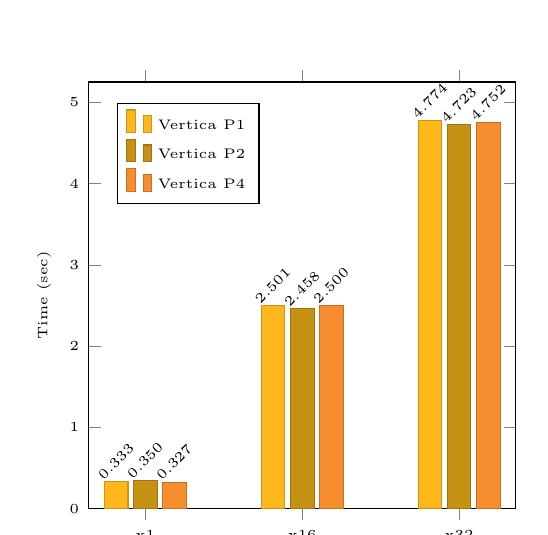
\begin{tikzpicture}
	\begin{axis}[
		symbolic x coords={x1, x16, x32},
		enlarge x limits=0.18,
		legend style={at={(0.4,0.95)}, anchor=north east},
		width = 7cm,
		height = 7cm
	]
	\addplot+ [bar width=0.3cm, ybar, color1!80!black, fill=color1, text=black] coordinates {(x1, 0.3334) (x16, 2.5006) (x32, 4.7736) };
	\addplot+ [bar width=0.3cm, ybar, color2!80!black, fill=color2, text=black] coordinates {(x1, 0.35) (x16, 2.4584) (x32, 4.7226) };
	\addplot+ [bar width=0.3cm, ybar, color3!80!black, fill=color3, text=black] coordinates {(x1, 0.3272) (x16, 2.4998) (x32, 4.7522) };
	\legend{Vertica P1, Vertica P2, Vertica P4}
	\end{axis}
	\end{tikzpicture}
		\caption{Vertica - 311 (Parallelism)}
		\label{fig:311ParallelismVertica}
	\end{minipage}%
	\begin{minipage}{.5\textwidth}
	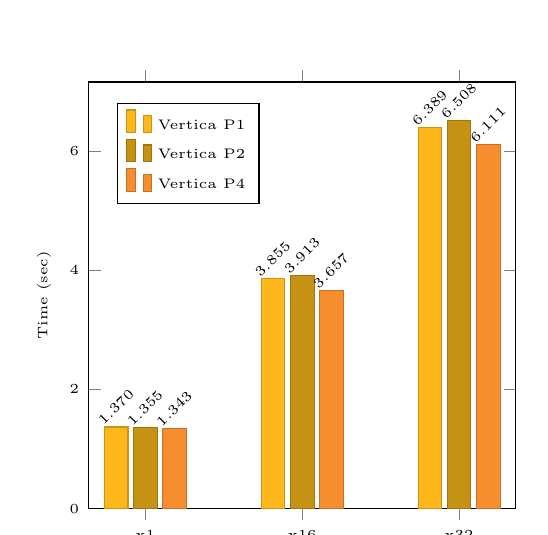
\begin{tikzpicture}
	\begin{axis}[
		symbolic x coords={x1, x16, x32},
		enlarge x limits=0.18,
		legend style={at={(0.4,0.95)}, anchor=north east},
		width = 7cm,
		height = 7cm
	]
	\addplot+ [bar width=0.3cm, ybar, color1!80!black, fill=color1, text=black] coordinates {(x1, 1.3702) (x16, 3.855) (x32, 6.3892) };
	\addplot+ [bar width=0.3cm, ybar, color2!80!black, fill=color2, text=black] coordinates {(x1, 1.3554) (x16, 3.9134) (x32, 6.5084) };
	\addplot+ [bar width=0.3cm, ybar, color3!80!black, fill=color3, text=black] coordinates {(x1, 1.3434) (x16, 3.6574) (x32, 6.1112) };
	\legend{Vertica P1, Vertica P2, Vertica P4}
	\end{axis}
	\end{tikzpicture}
		\caption{Vertica - Weblogs (Parallelism)}
		\label{fig:WeblogsParallelismVertica}
	\end{minipage}
	\end{figure}
	\begin{figure}[!ht]
	\begin{minipage}{.5\textwidth}
	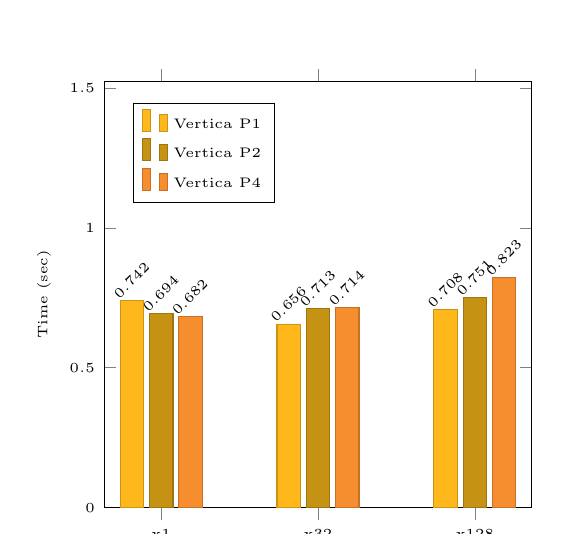
\begin{tikzpicture}
	\begin{axis}[
		symbolic x coords={x1, x32, x128},
		enlarge x limits=0.18,
		enlarge y limits=5.7,
		ymin=0.7,
		legend style={at={(0.4,0.95)}, anchor=north east},
		width = 7cm,
		height = 7cm
	]
	\addplot+ [bar width=0.3cm, ybar, color1!80!black, fill=color1, text=black] coordinates {(x1, 0.7416) (x32, 0.656) (x128, 0.7076) };
	\addplot+ [bar width=0.3cm, ybar, color2!80!black, fill=color2, text=black] coordinates {(x1, 0.6944) (x32, 0.7126) (x128, 0.7512) };
	\addplot+ [bar width=0.3cm, ybar, color3!80!black, fill=color3, text=black] coordinates {(x1, 0.6816) (x32, 0.714) (x128, 0.823) };
	\legend{Vertica P1, Vertica P2, Vertica P4}
	\end{axis}
	\end{tikzpicture}
		\caption{Vertica - Zillow1 (Parallelism)}
		\label{fig:Zillow1ParallelismVertica}
	\end{minipage}%
	\begin{minipage}{.5\textwidth}
	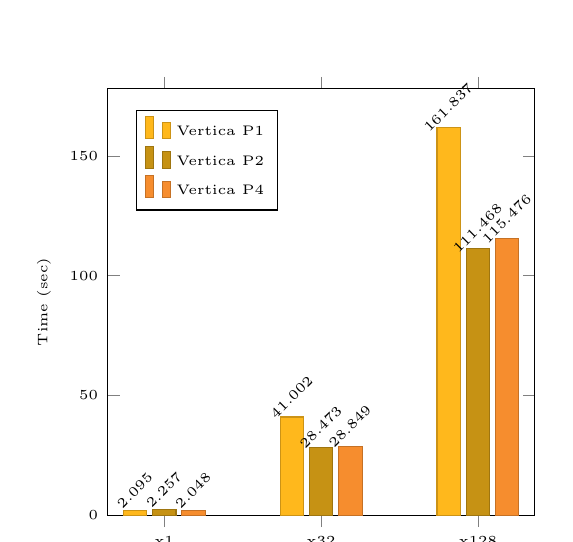
\begin{tikzpicture}
	\begin{axis}[
		symbolic x coords={x1, x32, x128},
		enlarge x limits=0.18,
		legend style={at={(0.4,0.95)}, anchor=north east},
		width = 7cm,
		height = 7cm
	]
	\addplot+ [bar width=0.3cm, ybar, color1!80!black, fill=color1, text=black] coordinates {(x1, 2.0954) (x32, 41.0024) (x128, 161.8368) };
	\addplot+ [bar width=0.3cm, ybar, color2!80!black, fill=color2, text=black] coordinates {(x1, 2.257) (x32, 28.473) (x128, 111.4684) };
	\addplot+ [bar width=0.3cm, ybar, color3!80!black, fill=color3, text=black] coordinates {(x1, 2.048) (x32, 28.8494) (x128, 115.4764) };
	\legend{Vertica P1, Vertica P2, Vertica P4}
	\end{axis}
	\end{tikzpicture}
		\caption{Vertica - Zillow2 (Parallelism)}
		\label{fig:Zillow2ParallelismVertica}
	\end{minipage}
	\end{figure}

\paragraph{MongoDB} in its native implementation, is capable 
of carrying query execution in parallel. 
Based on its original documentation~\cite{MogoDBConc}, mongod process uses a modified 
reader/writer lock with dynamic yielding on page faults
and long operations. Any number of concurrent 
read operations are allowed, but a write operation can block all 
other operation. 


can be the right choice for concurrency, 
as multi-granularity locking is used, which allows
operations to lock at the global, database or collection level. 
Additionally, for individual storage engines, it is allowed
to implement their own concurrency control below the collection level. 
In terms of compliance, pandas library was used, and the parallelism was done
on python level. In other words, we solve the problem of having 
a big dataframe, and one wants to apply a complex function to every 
record of this dataframe, which takes a lot of time. 
More specifically, we use a function~\ref{lst:paralDF} 
as proposed in this article~\cite{ParallelDF}, 
which breaks the dataframe into \emph{n\_cores} parts, 
and spawns \emph{n\_cores} processes which apply 
the function to all the pieces. Once 
Pool from multiprocessing 
library was used.
\begin{lstlisting}[language=Python, caption= {Kernel Parallelization in Python}, 
	label={lst:paralDF}]
	def parallelize_dataframe(df, func, n_cores=4):
		df_split = np.array_split(df, n_cores)
		pool = Pool(n_cores)
		df = pd.concat(pool.map(func, df_split))
		pool.close()
		pool.join()
		return df
\end{lstlisting}

	
\begin{figure}[t]
\begin{minipage}{.5\textwidth}
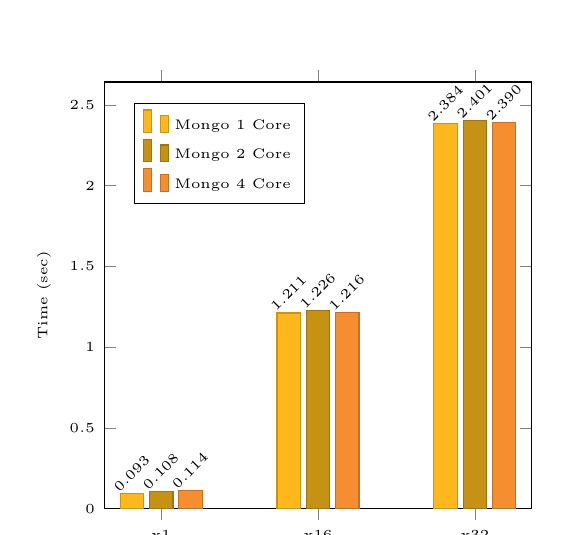
\begin{tikzpicture}
\begin{axis}[
	symbolic x coords={x1, x16, x32},
	enlarge x limits=0.18,
	legend style={at={(0.47,0.95)}, anchor=north east},
	width = 7cm,
	height = 7cm
]
\addplot+ [bar width=0.3cm, ybar, color1!80!black, fill=color1, text=black] coordinates {(x1, 0.0934848) (x16, 1.2112494) (x32, 2.3839544) };
\addplot+ [bar width=0.3cm, ybar, color2!80!black, fill=color2, text=black] coordinates {(x1, 0.1075664) (x16, 1.2260764) (x32, 2.4011928) };
\addplot+ [bar width=0.3cm, ybar, color3!80!black, fill=color3, text=black] coordinates {(x1, 0.113517) (x16, 1.215507) (x32, 2.3902328) };
\legend{Mongo 1 Core, Mongo 2 Core, Mongo 4 Core}
\end{axis}
\end{tikzpicture}
	\caption{Mongo - 311 (Parallelism)}
	\label{fig:311ParallelismMongo}
\end{minipage}%
\begin{minipage}{.5\textwidth}
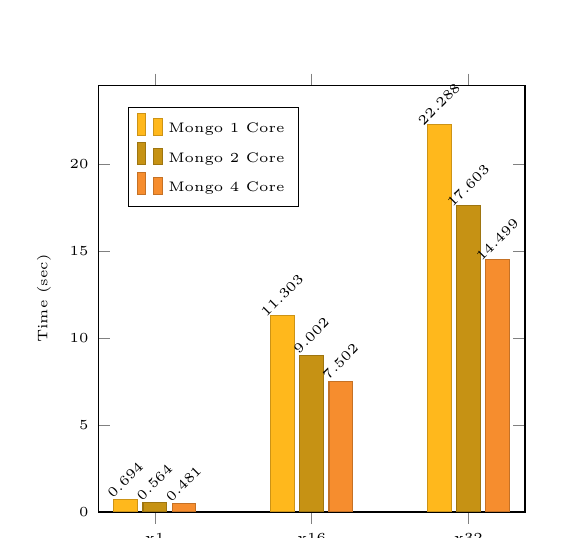
\begin{tikzpicture}
\begin{axis}[
	symbolic x coords={x1, x16, x32},
	enlarge x limits=0.18,
	legend style={at={(0.47,0.95)}, anchor=north east},
	width = 7cm,
	height = 7cm
]
\addplot+ [bar width=0.3cm, ybar, color1!80!black, fill=color1, text=black] coordinates {(x1, 0.6939822) (x16, 11.303007) (x32, 22.288301) };
\addplot+ [bar width=0.3cm, ybar, color2!80!black, fill=color2, text=black] coordinates {(x1, 0.564085) (x16, 9.0017266) (x32, 17.6031448) };
\addplot+ [bar width=0.3cm, ybar, color3!80!black, fill=color3, text=black] coordinates {(x1, 0.48111) (x16, 7.5024536) (x32, 14.4992794) };
\legend{Mongo 1 Core, Mongo 2 Core, Mongo 4 Core}
\end{axis}
\end{tikzpicture}
	\caption{Mongo - Weblogs (Parallelism)}
	\label{fig:WeblogsParallelismMongo}
\end{minipage}
\end{figure}
\begin{figure}[t]
\begin{minipage}{.5\textwidth}
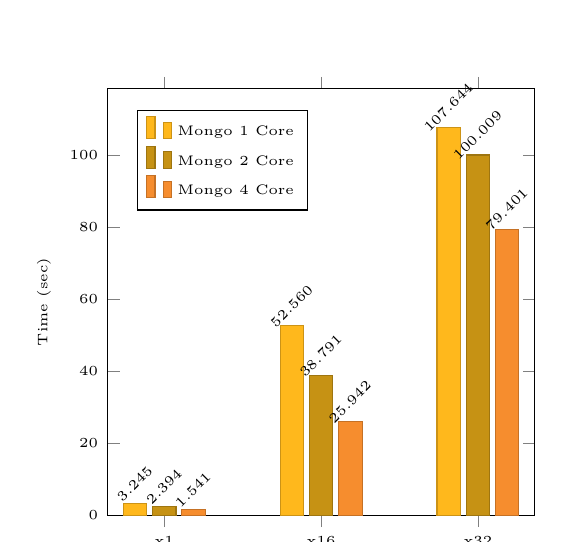
\begin{tikzpicture}
\begin{axis}[
	symbolic x coords={x1, x16, x32},
	enlarge x limits=0.18,
	legend style={at={(0.47,0.95)}, anchor=north east},
	width = 7cm,
	height = 7cm
]
\addplot+ [bar width=0.3cm, ybar, color1!80!black, fill=color1, text=black] coordinates {(x1, 3.2449956) (x16, 52.5604554) (x32, 107.6443716) };
\addplot+ [bar width=0.3cm, ybar, color2!80!black, fill=color2, text=black] coordinates {(x1, 2.3943826) (x16, 38.790527) (x32, 100.0086542) };
\addplot+ [bar width=0.3cm, ybar, color3!80!black, fill=color3, text=black] coordinates {(x1, 1.5410532) (x16, 25.9415926) (x32, 79.4014554) };
\legend{Mongo 1 Core, Mongo 2 Core, Mongo 4 Core}
\end{axis}
\end{tikzpicture}
	\caption{Mongo - Zillow1 (Parallelism)}
	\label{fig:Zillow1ParallelismMongo}
\end{minipage}%
\begin{minipage}{.5\textwidth}
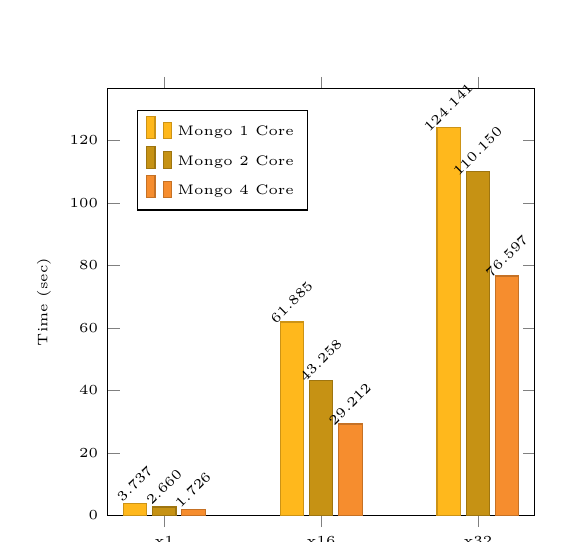
\begin{tikzpicture}
\begin{axis}[
	symbolic x coords={x1, x16, x32},
	enlarge x limits=0.18,
	legend style={at={(0.47,0.95)}, anchor=north east},
	width = 7cm,
	height = 7cm
]
\addplot+ [bar width=0.3cm, ybar, color1!80!black, fill=color1, text=black] coordinates {(x1, 3.7367452) (x16, 61.8848998) (x32, 124.1408488) };
\addplot+ [bar width=0.3cm, ybar, color2!80!black, fill=color2, text=black] coordinates {(x1, 2.6603464) (x16, 43.2579538) (x32, 110.1501846) };
\addplot+ [bar width=0.3cm, ybar, color3!80!black, fill=color3, text=black] coordinates {(x1, 1.7257306) (x16, 29.2115762) (x32, 76.596979) };
\legend{Mongo 1 Core, Mongo 2 Core, Mongo 4 Core}
\end{axis}
\end{tikzpicture}
	\caption{Mongo - Zillow2 (Parallelism)}
	\label{fig:Zillow2ParallelismMongo}
\end{minipage}
\end{figure}
\section{Discussion}
\label{sec:discussion}

%TODO
% Figures 1-4: 
% * column based faster (+Vertica and monetdb measurements outperforms others)
% * no significant improvements in hot and cold as expected (+citation)
% * queries: 
%     - zillow1: many nested calls
%     - Weblogs: join 
%     - zillow2, 311 aggregated
% * size of data differences: linear increase
% * postgres parallelism: no difference independently the query 
%     + reasons: query plan execution, #data, hardware
% * monetdb: same
% * vertica, only zillow2 (many aggregations), followed by weblogs which has join
%     - no difference on nested queries
% * mongodb: 
%     - 311 distinct -> logically no difference, same 250 to applyUDF -> 
%     - weblogs, zillow1, zillow2: applyUDF and every time splits data in more partitions 
%         (-) implementation has no safeguard on how many cores will be utilized
%     - native mongo much better (i.e. weblogs)


\section{Threats to validity }
\label{sec:threats}

%TODO
% Single node running
\section{Conclusion}
\label{sec:conclusion}





\printbibliography[heading=bibintoc]
\label{bib:bib}


% \clearpage
\setcounter{page}{1}
% \appendix
% \setcounter{secnumdepth}{0}
%\input{sections/appendix.tex}
% \clearpage
% \input{sections/appendixB.tex}


\end{document}
